\chapter{Causal Models}
In un \textbf{randomized control experiment} tutti i fattori $X_1, ..., X_n$ che influenzano l'outcome $Y$ sono statici o variati randomicamente tranne uno  $X_i$.
In questo modo un cambiamento nell'outcome $Y$ sarà dovuto solo da quel fattore $X_i$.

Spesso non è possibile effettuare gli esperimenti per cause pratiche o etiche, quindi si eseguono degli studi osservazionali in un cui
si raccolgono i dati rispetto ad alterarli.

Il problema degli studi osservazionali è distinguere la causazione dalla correlazione.

\section{Intervention and do-Operator}
\begin{center}
  \begin{minipage}{0.475\linewidth}
    \centering
    \textbf{Intervening}

    Cambiamo il sistema fissando $X=x$ e osserviamo i cambiamenti su tutta la popolazione.
  \end{minipage}
  \begin{minipage}{0.475\linewidth}
    \centering
    \textbf{Conditioning}

    Non cambiamo nulla e consideriamo un sottoinsieme della popolazione $X=x$.
  \end{minipage}
\end{center}

Denotiamo l'intervention con il do-operator $do(X=x)$.
\begin{align*}
  P(Y(x) = y) = P(Y = y | do(X = x)) = P(y | do(x))
\end{align*}
%
\begin{align*}
   & P(Y | X = x) = P(y | x)         \qquad & \text{observational distribution}  \\
   & P(Y | do(X = x)) = P(y | do(x)) \qquad & \text{interventional distribution}
\end{align*}

Un'espressione con $do$ è detta interventional expression, mentre senza $do$ è detta observational expression.

Un'interventional expression che può essere ridotta a una observational expression è detta \textbf{identificabile}.

Una stima è detta causale se contiene il do-operator, statistica altrimenti.

\bigskip
\begin{center}
  \begin{minipage}{0.475\linewidth}
    \centering
    \textbf{pre-intervention distribution}
    \begin{align*}
      P(Y | do(x), Z = z)
    \end{align*}
  \end{minipage}
  \begin{minipage}{0.475\linewidth}
    \centering
    \textbf{post-intervention distribution}
    \begin{align*}
      P(Y | x, Z = z)
    \end{align*}
  \end{minipage}
\end{center}
\bigskip

\section{Modularity and Adjustment Formula}
Il \textbf{causal mechanism} è un meccanismo che genera $X_i$ come distribuzione condizionale di $X_i$ dati i genitori (cause) $pa(X_i)$, ovvero $P(X_i | pa(X_i))$.

Assunzione: Le intervention sono locali

Un intervention su una variabile $X_i$ cambia solo il suo causal mechanism, non cambia il causal mechanism che genera un'altra variabile $X_j$.

\subsection*{Modularity - Independence Mechanism - Invariance}
Se interveniamo su un insieme di variabili $S$ fissando valori costanti,
allora per ogni variabile $X_i \in \{X_1, ..., X_n\}$ possiamo affermare che:
\begin{enumerate}
  \item Se $X_i \in S$, allora $P(X_i = x| pa(X_i)) = 1$ se $x$ è il valore assegnato dall'intervention $do(X_i=x)$, 0 altrimenti
  \item Se $X_i \not\in S$, allora $P(X_i = x | pa(X_i))$ rimane inalterato
\end{enumerate}

Data una variabile $X_i \in S$, un valore $x$ di $X_i$ è \textbf{consistente} con l'intervention su $X_i$ se $x$ è uguale al valore che è stato assegnato nell'intervention $do(X_i=x)$.

Una volta impostato il valore di $X_i$ non importa più il valore dei nodi genitori $pa(X_i)$, poiché al variare di $pa(X_i)$ non varierà il valore di $X_i$.

Questo possiamo rappresentarlo attraverso un grafo (detto manipulated graph o \textbf{post-intervention graph}) in cui si rimuoviamo gli archi entranti in $X_i$; se non ce ne sono, vuol dire che l'intervention non ha conseguenze sulla distribuzione post-intervention
$p(y|do(x)) = p(y|x)$.

\subsection*{Adjustment Formula}
Dato il seguente grafo causale e il suo corrispettivo grafo manipolato a seguito dell'intervention sulla variabile $X$.

\begin{center}
  \begin{minipage}{0.4\linewidth}
    \centering
    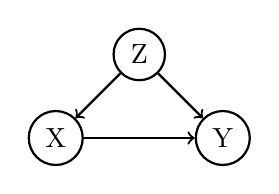
\begin{tikzpicture}[node distance={15mm}, thick, main/.style = {draw, circle}]
      \node[main] (1) {Z};
      \node[main] (2) [below right of=1] {Y};
      \node[main] (3) [below left of=1] {X};
      \draw[->] (1) -- (2);
      \draw[->] (1) -- (3);
      \draw[->] (3) -- (2);
    \end{tikzpicture}

    pre-intervention graph
  \end{minipage}
  %
  {\Large$\overset{do(X = x)}{\Longrightarrow}$}
  %
  \begin{minipage}{0.4\linewidth}
    \centering
    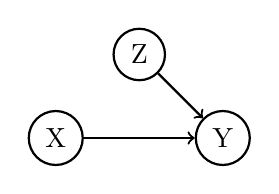
\begin{tikzpicture}[node distance={15mm}, thick, main/.style = {draw, circle}]
      \node[main] (1) {Z};
      \node[main] (2) [below right of=1] {Y};
      \node[main] (3) [below left of=1] {X};
      \draw[->] (1) -- (2);
      \draw[->] (3) -- (2);
    \end{tikzpicture}

    post-intervention graph
  \end{minipage}
\end{center}

Possiamo osservare sotto la condizione di \textbf{modularity assumption} che:
\begin{enumerate}
  \item $P(Y = y|do(X = x)) = Pm (Y = y|X = x)$
  \item $P(Z|do(X=x)) = P_m(Z|x) = P(Z)$
  \item $P(Y|do(X=x), Z) = P_m(Y|x,Z) = P(Y|x,Z)$
\end{enumerate}

La probabilità marginale $P(Z)$ e la probabilità condizionale $P(Y|x,Z)$ sono invarianti all'intervention.
Questo perché il causal mechanism di X non influenza il causal mechanism delle altre variabili.

Date le seguenti uguaglianze:

\begin{enumerate}
  \item $P_m(Z=z | X=x) = P_m(Z=z) = P(Z=z)$
  \item $P_m(Y=y|X=x, Z=z) = P(Y=y|X=x, Z=z)$
\end{enumerate}

Possiamo scrivere la seguente interventional expression:
\begin{align*}
  P(Y=y|do(X=x)) & = P_m(Y=y|X=x)                            \\
                 & = \sum_z P_m(Y=y|X=x, Z=z) P_m(Z=z | X=x) \\
                 & = \sum_z P_m(Y=y|X=x, Z=z) P_m(Z=z)       \\
                 & = \sum_z P(Y=y|X=x, Z=z) P(Z=z)
\end{align*}

Il causal mechanism di $Y$,  $P(Y=y|X=x, Z=z)$ viene aggiustato, pesato da $Z$ (adjusting/controlling for $Z$).

Quest'espressione prende il nome di Adjustment Formula e ci permette di rispondere a una interventional query solo usando 
dati osservazionali. 

\subsection*{Causal Effect Rule}
Generalizzazione della adjustment formula.

Dato un grafo $G$ in cui un insieme di variabili $pa(X)$ sono i genitori di $X$
\begin{align*}
  P(Y=y | do(X=x)) & = \sum_u {P(Y=y | X=x, pa(X)=u) P(pa(X)=u)}              \\
                   & = \sum_u {\frac{P(Y=y, X=x, pa(X)=u)}{P(X=x | pa(X)=u)}}
\end{align*}

\section{Backdoor Adjustment}
